% This LaTeX document needs to be compiled with XeLaTeX.
\documentclass[10pt]{article}
\usepackage[utf8]{inputenc}
\usepackage{amsmath}
\usepackage{amsfonts}
\usepackage{amssymb}
\usepackage[version=4]{mhchem}
\usepackage{stmaryrd}
\usepackage{graphicx}
\usepackage[export]{adjustbox}
\graphicspath{ {./images/} }
\usepackage{multirow}
\usepackage[fallback]{xeCJK}
\usepackage{polyglossia}
\usepackage{fontspec}
\setCJKmainfont{Noto Serif CJK TC}

\setmainlanguage{polish}
\setmainfont{CMU Serif}

\title{Instrukcja dla zdającego }

\author{}
\date{}


\newcommand\Varangle{\mathop{{<\!\!\!\!\!\text{\small)}}\:}\nolimits}

\begin{document}
\maketitle
Czas pracy:

\begin{enumerate}
  \item Sprawdź, czy arkusz zawiera 16 stron.
  \item Rozwiązania zadań i odpowiedzi zamieść w miejscu na to przeznaczonym.
  \item W zadaniach od 1 do 25 są podane 4 odpowiedzi: A, B, C, D, z których tylko jedna jest prawdziwa. Wybierz tylko jedną odpowiedź i zaznacz ją na karcie odpowiedzi.
  \item Zaznaczając odpowiedzi w części karty przeznaczonej dla zdającego, zamaluj pola do tego przeznaczone. Błędne zaznaczenie otocz kółkiem i zaznacz właściwe.
  \item Rozwiązania zadań od 26 do 34 zapisz starannie i czytelnie w wyznaczonych miejscach. Przedstaw swój tok rozumowania prowadzący do ostatecznego wyniku.
  \item Pamiętaj, że pominięcie argumentacji lub istotnych obliczeń w rozwiązaniu zadania otwartego może spowodować, że za to rozwiązanie możesz nie dostać pełnej liczby punktów.
  \item Pisz czytelnie. Używaj długopisu/pióra tylko z czarnym tuszem/atramentem.
  \item Nie używaj korektora. Błędne zapisy przekreśl.
  \item Pamiętaj, że zapisy w brudnopisie nie podlegają ocenie.
  \item Obok numeru każdego zadania podana jest maksymalna liczba punktów możliwych do uzyskania.
  \item Możesz korzystać z zestawu wzorów matematycznych, cyrkla i linijki oraz kalkulatora.
  \item Wypełnij tę częşć karty odpowiedzi, którą koduje zdający. Nie wpisuj żadnych znaków części przeznaczonej dla egzaminatora.
\end{enumerate}

Liczba\\
punktów\\
do\\
uzyskania:\\
50

\section*{ZADANIA ZAMKNIETE}
W zadaniach o numerach od 1 do 25 wybierz i zaznacz na karcie odpowiedzi jedną poprawną odpowiedź.

Zadanie 1. (1pkt)\\
Dane są zbiory: \(A=\langle-5 ; 3)\) oraz \(B=\langle 2 ; 7)\). Zbiór \(A \cap B\) zaznaczony jest na rysunku:\\
A.\\
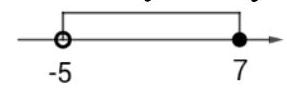
\includegraphics[max width=\textwidth, center]{2024_11_21_55bf50695fa934dbe20eg-02(2)}\\
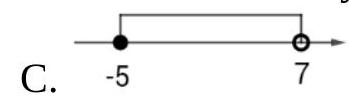
\includegraphics[max width=\textwidth, center]{2024_11_21_55bf50695fa934dbe20eg-02}\\
D.\\
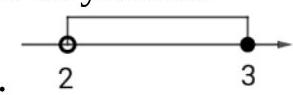
\includegraphics[max width=\textwidth, center]{2024_11_21_55bf50695fa934dbe20eg-02(1)}

Zadanie 2. (1pkt)\\
Liczba \(||4-7|-|13-5||\) jest równa:\\
A. 5\\
B. 7\\
C. 11\\
D. 29

Zadanie 3. (1pkt)\\
Odwrotnością liczby \(2 \sqrt{2}-3\) jest liczba:\\
A. \(-3-2 \sqrt{2}\)\\
B. \(2 \sqrt{2}+3\)\\
C. \(\frac{1}{2 \sqrt{2}+3}\)\\
D. \(3-2 \sqrt{2}\)

Zadanie 4. (1pkt)\\
Liczba \(\sqrt[3]{9^{6} \cdot\left(\frac{1}{3}\right)^{9}: 27^{-1}}\) jest równa:\\
A. \(3^{8}\)\\
B. \(3^{6}\)\\
C. \(3^{0}\)\\
D. \(3^{2}\)

Zadanie 5. (1pkt)\\
Liczba \(-2 \log _{3} 6+3 \log _{3} 2\) jest równa:\\
A. \(\log _{3} \frac{1}{18}\)\\
B. \(\log _{3} 288\)\\
C. \(\log _{3} \frac{2}{9}\)\\
D. -1

Zadanie 6. (1pkt)\\
Liczba \(\sqrt{128}-0,5 \sqrt{32}\) jest równa:\\
A. \(\sqrt{112}\)\\
B. \(\sqrt{8}\)\\
C. \(4 \sqrt{2}\)\\
D. \(6 \sqrt{2}\)

\section*{Zadanie 7. (1pkt)}
Koszt uczestnictwa w obozie sportowym w 2018 r. wynosi 1620 zł. Wzrósł on w stosunku do kosztu z 2017 r. o 35\%. Koszt uczestnictwa w obozie w 2017 r. wynosił:\\
A. \(567 \mathrm{zł}\)\\
B. 1200 zt\\
C. 1053 zt\\
D. 1215 zf

\section*{Zadanie 8. (1pkt)}
Wartość wyrażenia \(\left(-1-x^{3}\right)\left(x^{3}-1\right)\) dla \(x=-\sqrt[3]{3}\) jest równa:\\
A. -2\\
B. 2\\
C. -8\\
D. -4

Zadanie 9. (1pkt)\\
Do zbioru rozwiązań równania \(x(x+2)\left(x^{2}-1\right)=0\) nie należy liczba:\\
A. 2\\
B. 1\\
C. 0\\
D. -1

Zadanie 10. (1pkt)\\
Wartość wyrażenia \((4-\sqrt{3})^{2}-(4+\sqrt{3})^{2}\) wynosi:\\
A. 6\\
B. \(-16 \sqrt{3}\)\\
C. \(-4 \sqrt{3}\)\\
D. -6

Zadanie 11. (1pkt)\\
Marta oszacowała, że wyda na zakupy około 50 zł. W rzeczywistości zapłaciła 48 zł. Błąd względny, jaki popełniła szacując wartość zakupów wynosi:\\
A. \(\frac{2}{25}\)\\
B. 2\\
C. \(\frac{1}{24}\)\\
D. \(\frac{1}{25}\)

Zadanie 12. (1pkt)\\
Dany jest zbiór \(A=\left\{\frac{\pi}{2} ;-1 ; \sqrt{7 \frac{1}{9}} ; 0 ; 1\right.\), (3) \(\left.; \frac{1-\sqrt{3}}{4}\right\}\). Liczb wymiernych w zbiorze A jest:\\
A. pięć\\
B. trzy\\
C. cztery\\
D. dwie

Zadanie 13. (1pkt)\\
Układ równań \(\left\{\begin{array}{c}3 x-4 y=5 \\ -6 x+(a+3) y=10\end{array}\right.\) jest sprzeczny dla:\\
A. \(a=-2\)\\
B. \(a=-11\)\\
C. \(a=3\)\\
D. \(a=5\)

Zadanie 14. (1pkt)\\
Odcinek AB jest średnicą okręgu (rysunek).\\
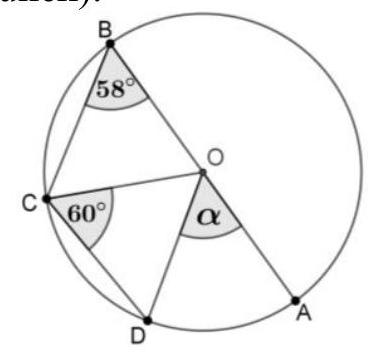
\includegraphics[max width=\textwidth, center]{2024_11_21_55bf50695fa934dbe20eg-04}

Miara kąta \(\alpha\) jest równa:\\
A. \(56^{\circ}\)\\
B. \(116^{\circ}\)\\
C. \(58^{\circ}\)\\
D. \(60^{\circ}\)

Zadanie 15. (1pkt)\\
Długości boków trójkąta nie mogą być równe:\\
A. \(3 ; 4 ; 4\)\\
B. \(3 ; 4 ; 8\)\\
C. \(3 ; 4 ; 5\)\\
D. \(3 ; 4 ; 2\)

\section*{Zadanie 16. (1pkt)}
Dwa boki trójkąta prostokątnego mają długości 3 cm oraz 4 cm . Długość najkrótszego boku tego trójkąta wynosi:\\
A. 5 cm\\
B. \(2,6 \mathrm{~cm}\)\\
C. \(\sqrt{5} \mathrm{~cm}\)\\
D. \(\sqrt{7} \mathrm{~cm}\)

Zadanie 17. (1pkt)\\
Pole koła opisanego na trójkącie prostokątnym o bokach długości 10, 24, 26 jest równe:\\
A. \(169 \pi\)\\
B. \(26 \pi\)\\
C. \(144 \pi\)\\
D. \(25 \pi\)

Zadanie 18. (1pkt)\\
Trójkąty ABC oraz A'B'C' są podobne. Obwód trójkąta A'B'C' jest równy 12, a jego pole 6.\\
Jeżeli pole trójkąta ABC jest równe \(13 \frac{1}{2}\), to jego obwód wynosi:\\
A. \(6 \frac{3}{4}\)\\
B. 27\\
C. 18\\
D. 9

Zadanie 19. (1pkt)\\
Na końcowym ramieniu kąta \(\alpha\) (rysunek) leży punkt \(\mathrm{P}=(-3 ; 4)\).\\
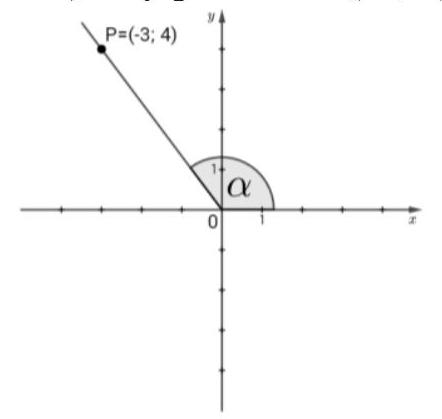
\includegraphics[max width=\textwidth, center]{2024_11_21_55bf50695fa934dbe20eg-06}

Wówczas:\\
A. \(\operatorname{tg} \alpha=\frac{4}{3}\)\\
B. \(\cos \alpha=-\frac{3}{5}\)\\
C. \(\sin \alpha=-\frac{3}{5}\)\\
D. \(\cos \alpha=-\frac{4}{3}\)

Zadanie 20. (1pkt)\\
Długość boku AC w trójkącie przedstawionym na poniższym rysunku jest równa:\\
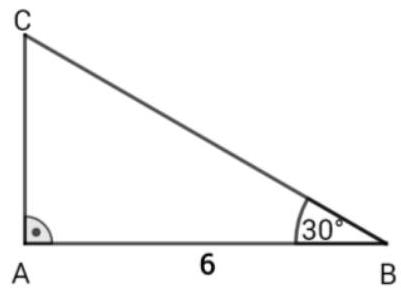
\includegraphics[max width=\textwidth, center]{2024_11_21_55bf50695fa934dbe20eg-06(1)}\\
A. \(3 \sqrt{2}\)\\
B. 3\\
C. \(2 \sqrt{3}\)\\
D. \(6 \sqrt{3}\)

Zadanie 21. (1pkt)\\
Wartość wyrażenia \(\cos 120^{\circ} \cdot \operatorname{tg} 120^{\circ}\) wynosi:\\
A. \(\frac{\sqrt{3}}{2}\)\\
B. \(\frac{1}{2}\)\\
C. 1\\
D. \(-\frac{\sqrt{3}}{2}\)

Zadanie 22. (1pkt)\\
Długość okręgu wpisanego w trójkąt równoboczny wynosi \(6 \pi\). Długość boku tego trójkąta jest równa:\\
A. \(2 \sqrt{3}\)\\
B. 6\\
C. 9\\
D. \(6 \sqrt{3}\)

Zadanie 23. (1pkt)\\
Zbiór \(\boldsymbol{R} \backslash\{3\}\) jest dziedziną funkcji:\\
A. \(f(x)=x-3\)\\
B. \(f(x)=\frac{x}{(x-3)^{2}}\)\\
C. \(f(x)=\frac{2}{x^{2}-9}\)\\
D. \(f(x)=\frac{x+3}{x^{2}-3}\)

Zadanie 24. (1pkt)\\
Do wykresu funkcji \(f(x)=2 \sqrt{3} x-4\) należy punkt o współrzędnych:\\
A. \((2 \sqrt{3} ; 2)\)\\
B. \((-4 ; 0)\)\\
C. \((-\sqrt{3} ;-10)\)\\
D. \((\sqrt{3} ;-2)\)

\section*{Zadanie 25. (1pkt)}
Wykres funkcji \(f(x)=(x-3)^{2}\) przesunięto równolegle o 2 jednostki w prawo. W wyniku tego przekształcenia otrzymano wykres funkcji:\\
A. \(g(x)=(x-3)^{2}+2\)\\
B. \(g(x)=(x-1)^{2}\)\\
C. \(g(x)=(x-3)^{2}-2\)\\
D. \(g(x)=(x-5)^{2}\)

\section*{ZADANIA OTWARTE}
Rozwiązania zadań o numerach od 26 do 34 należy zapisać w wyznaczonych miejscach pod treścią zadania.\\
Zadanie 26. (2 pkt)\\
Rozwiąż równanie \((x-3)^{2}-1=(x-2)(x+2)\).\\

\includegraphics[max width=\textwidth, center]{2024_11_21_55bf50695fa934dbe20eg-08}

Zadanie 27. (2 pkt)\\
Wykaż, że jeżeli \(a+b=4\), to \(a^{2}+b^{2} \geq 8\).

\begin{center}
\begin{tabular}{|c|c|c|c|c|c|c|c|c|c|c|c|c|c|c|c|c|c|c|c|c|c|c|c|c|c|c|c|c|c|c|c|}
\hline
 &  &  &  &  &  &  &  &  &  &  &  &  &  &  & \textbackslash  & 的 & 的 &  & ( & \textbackslash  & 的 & \textbackslash  & \textbackslash  & \textbackslash  & 的 & 的 &  &  &  &  &  \\
\hline
 &  &  &  &  &  &  &  &  &  &  &  &  &  &  &  &  &  &  &  &  &  &  &  &  &  &  &  &  &  &  &  \\
\hline
 &  &  &  &  &  &  &  &  &  &  &  &  &  &  &  &  &  &  &  &  &  &  &  &  &  &  &  &  &  &  &  \\
\hline
 &  &  &  &  &  &  &  &  &  &  &  &  &  &  &  &  &  &  &  &  &  &  &  &  &  &  &  &  &  &  &  \\
\hline
 &  &  &  &  &  &  &  &  &  &  &  &  &  &  &  &  &  &  &  &  &  &  &  &  &  &  &  &  &  &  &  \\
\hline
 &  &  &  &  &  &  &  &  &  &  &  &  &  &  &  &  &  &  &  &  &  &  &  &  &  &  &  &  &  &  &  \\
\hline
 &  &  &  &  &  &  &  &  &  &  &  &  &  &  &  &  &  &  &  &  &  &  &  &  &  &  &  &  &  &  &  \\
\hline
 &  &  &  &  &  &  &  &  &  &  &  &  &  &  &  &  &  &  &  &  &  &  &  &  &  &  &  &  &  &  &  \\
\hline
 &  &  &  &  &  &  &  &  &  &  &  &  &  &  &  &  &  &  &  &  &  &  &  &  &  &  &  &  &  &  &  \\
\hline
 &  &  &  &  &  &  &  &  &  &  &  &  &  &  &  &  &  &  &  &  &  &  &  &  &  &  &  &  &  &  &  \\
\hline
 &  &  &  &  &  &  &  &  &  &  &  &  &  &  &  &  &  &  &  &  &  &  &  &  &  &  &  &  &  &  &  \\
\hline
 &  &  &  &  &  &  &  &  &  &  &  &  &  &  &  &  &  &  &  &  &  &  &  &  &  &  &  &  &  &  &  \\
\hline
 &  &  &  &  &  &  &  &  &  &  &  &  &  &  &  &  &  &  &  &  &  &  &  &  &  &  &  &  &  &  &  \\
\hline
 &  &  &  &  &  &  &  &  &  &  &  &  &  &  &  &  &  &  &  &  &  &  &  &  &  &  &  &  &  &  &  \\
\hline
 &  &  &  &  &  &  &  &  &  &  &  &  &  &  &  &  &  &  &  &  &  &  &  &  &  &  &  &  &  &  &  \\
\hline
 &  &  &  &  &  &  &  &  &  &  &  &  &  &  &  &  &  &  &  &  &  &  &  &  &  &  &  &  &  &  &  \\
\hline
 &  &  &  &  &  &  &  &  &  &  &  &  &  &  &  &  &  &  &  &  &  &  &  &  &  &  &  &  &  &  &  \\
\hline
 &  &  &  &  &  &  &  &  &  &  &  &  &  &  &  &  &  &  &  &  &  &  &  &  &  &  &  &  &  &  &  \\
\hline
 &  &  &  &  &  &  &  &  &  &  &  &  &  &  &  &  &  &  &  &  &  &  &  &  &  &  &  &  &  &  &  \\
\hline
 &  &  &  &  &  &  &  &  &  &  &  &  &  &  &  &  &  &  &  &  &  &  &  &  &  &  &  &  &  &  &  \\
\hline
\end{tabular}
\end{center}

Zadanie 28. (2 pkt)\\
Kąt \(\alpha\) jest ostry i \(\cos \alpha=\frac{\sqrt{5}}{3}\). Oblicz wartość wyrażenia: \(\sin ^{3} \alpha-3 \cos ^{2} \alpha\).

\begin{center}
\begin{tabular}{|c|c|c|c|c|c|c|c|c|c|c|c|c|c|c|c|c|c|c|c|c|c|c|c|c|c|c|c|c|c|c|}
\hline
 &  &  &  &  &  &  &  &  &  &  &  &  &  &  &  &  &  &  &  &  &  &  &  &  &  &  &  &  &  &  \\
\hline
 &  &  &  &  &  &  &  &  &  &  &  &  &  &  &  &  &  &  &  &  &  &  &  &  &  &  &  &  &  &  \\
\hline
 &  &  &  &  &  &  &  &  &  &  &  &  &  &  &  &  &  &  &  &  &  &  &  &  &  &  &  &  &  &  \\
\hline
 &  &  &  &  &  &  &  &  &  &  &  &  &  &  &  &  &  &  &  &  &  &  &  &  &  &  &  &  &  &  \\
\hline
 &  &  &  &  &  &  &  &  &  &  &  &  &  &  &  &  &  &  &  &  &  &  &  &  &  &  &  &  &  &  \\
\hline
 &  &  &  &  &  &  &  &  &  &  &  &  &  &  &  &  &  &  &  &  &  &  &  &  &  &  &  &  &  &  \\
\hline
 &  &  &  &  &  &  &  &  &  &  &  &  &  &  &  &  &  &  &  &  &  &  &  &  &  &  &  &  &  &  \\
\hline
 &  &  &  &  &  &  &  &  &  &  &  &  &  &  &  &  &  &  &  &  &  &  &  &  &  &  &  &  &  &  \\
\hline
 &  &  &  &  &  &  &  &  &  &  &  &  &  &  &  &  &  &  &  &  &  &  &  &  &  &  &  &  &  &  \\
\hline
 &  &  &  &  &  &  &  &  &  &  &  &  &  &  &  &  &  &  &  &  &  &  &  &  &  &  &  &  &  &  \\
\hline
 &  &  &  &  &  &  &  &  &  &  &  &  &  &  &  &  &  &  &  &  &  &  &  &  &  &  &  &  &  &  \\
\hline
 &  &  &  &  &  &  &  &  &  &  &  &  &  &  &  &  &  &  &  &  &  &  &  &  &  &  &  &  &  &  \\
\hline
 &  &  &  &  &  &  &  &  &  &  &  &  &  &  &  &  &  &  &  &  &  &  &  &  &  &  &  &  &  &  \\
\hline
 &  &  &  &  &  &  &  &  &  &  &  &  &  &  &  &  &  &  &  &  &  &  &  &  &  &  &  &  &  &  \\
\hline
 &  &  &  &  &  &  &  &  &  &  &  &  &  &  &  &  &  &  &  &  &  &  &  &  &  &  &  &  &  &  \\
\hline
 &  &  &  &  &  &  &  &  &  &  &  &  &  &  &  &  &  &  &  &  &  &  &  &  & 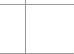
\includegraphics[max width=\textwidth]{2024_11_21_55bf50695fa934dbe20eg-09}
 &  &  &  &  &  \\
\hline
 &  &  &  &  &  &  &  &  &  &  &  &  &  &  &  &  &  &  &  &  &  &  &  &  &  &  &  &  &  &  \\
\hline
 &  &  &  &  &  &  &  &  &  &  &  &  &  &  &  &  &  &  &  &  &  &  &  &  &  &  &  &  &  &  \\
\hline
 &  &  &  &  &  &  &  &  &  &  &  &  &  &  &  &  &  &  &  &  &  &  &  &  &  &  &  &  &  &  \\
\hline
\end{tabular}
\end{center}

Zadanie 29. (2 pkt)\\
Trójkąt ABC jest prostokątny. Z punktu K należącego do przeciwprostokątnej AB poprowadzono odcinki KM oraz KL prostopadłe odpowiednio do przyprostokątnych BC ora AC (rysunek).\\
Wykaż, że \(\frac{|K M|}{|A C|}+\frac{|K L|}{|B C|}=1\).\\

\includegraphics[max width=\textwidth, center]{2024_11_21_55bf50695fa934dbe20eg-09(1)}

Zadanie 30. (2 pkt)\\
W trójkącie ABC dane są: \(|A B|=|B C|=6\) oraz \(|\Varangle A B C|=45^{\circ}\). Oblicz długość wysokości tego trójkąta poprowadzonej z wierzchołka C.\\

\includegraphics[max width=\textwidth, center]{2024_11_21_55bf50695fa934dbe20eg-10(1)}

Zadanie 31. (2 pkt)\\
Odcinki \(A B\) oraz \(A C\) (rysunek) są równej długości. Kąt CAB ma miarę o \(116^{\circ}\) mniejszą od miary kąta do niego przyległego. Oblicz miarę kąta BCD.\\

\includegraphics[max width=\textwidth, center]{2024_11_21_55bf50695fa934dbe20eg-10}

Zadanie 32. (5 pkt)\\
Poniżej przedstawiony jest wykres funkcji \(y=f(x)\). Na podstawie tego wykresu podaj:\\
a) dziedzinę funkcji \(f\),\\
b) zbiór wartości funkcji \(f\),\\
c) maksymalne przedziały, w których funkcja \(f\) jest rosnąca,\\
d) miejsca zerowe funkcji \(f\),\\
e) zbiór argumentów, dla których funkcja \(f\) przyjmuje wartości niedodatnie.\\
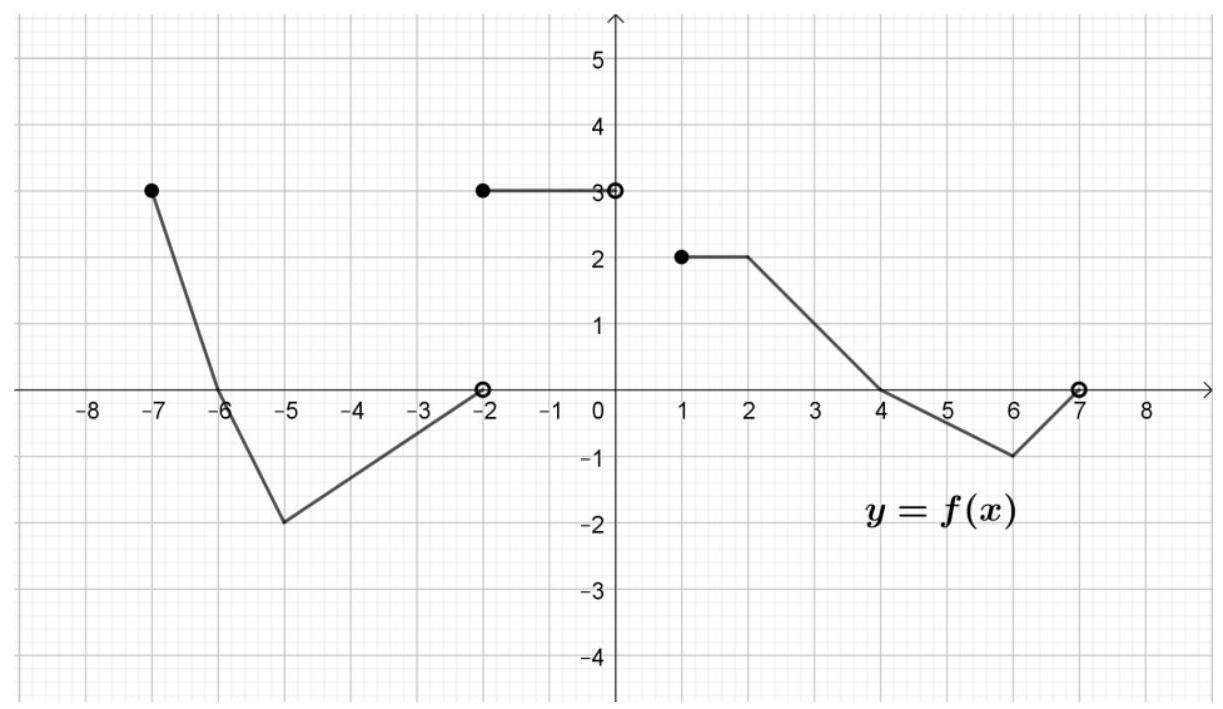
\includegraphics[max width=\textwidth, center]{2024_11_21_55bf50695fa934dbe20eg-11}\\

\includegraphics[max width=\textwidth, center]{2024_11_21_55bf50695fa934dbe20eg-11(1)}

Zadanie 33. (4 pkt)\\
Marcin zarabiał miesięcznie 3400 zł, a Adam 4300 zł. Obaj otrzymali w swoich firmach podwyżki. Podwyżka otrzymana przez Adama była o 4 punkty procentowe niższa niż podwyżka otrzymana przez Marcina. Po podwyżce obaj panowie zarabiają łącznie 8452 zł. Ile zarabia każdy z panów po podwyżce? Zapisz wszystkie obliczenia.\\

\includegraphics[max width=\textwidth, center]{2024_11_21_55bf50695fa934dbe20eg-12}

Zadanie 34. (4 pkt)\\
Wyznacz wszystkie liczby pierwsze, które należą do zbioru \(A \backslash B\), gdzie \(A\) jest zbiorem rozwiązań nierówności:

\[
\left(\log _{4} 24-\log _{4} 6\right)+3 x \geq-7-x
\]

a \(B\) jest zbiorem rozwiązań nierówności:

\[
3-\frac{x-1}{2}<-3
\]

\begin{center}
\begin{tabular}{|c|c|c|c|c|c|c|c|c|c|c|c|c|c|c|c|c|c|c|c|c|c|c|c|}
\hline
 &  &  &  &  &  &  &  &  &  &  &  &  &  &  &  &  &  &  &  &  &  &  &  \\
\hline
 &  &  &  &  &  &  &  &  &  &  &  &  &  &  &  &  &  &  &  &  &  &  &  \\
\hline
 &  &  &  &  &  &  &  &  &  &  &  &  &  &  &  &  &  &  &  &  &  &  &  \\
\hline
 &  &  &  &  &  &  &  &  &  &  &  &  &  &  &  &  &  &  &  &  &  &  &  \\
\hline
 &  &  &  &  &  &  &  &  &  &  &  &  &  &  &  &  &  &  &  &  &  &  &  \\
\hline
 &  &  &  &  &  &  &  &  &  &  &  &  &  &  &  &  &  &  &  &  &  &  &  \\
\hline
 &  &  &  &  &  &  &  &  &  &  &  &  &  &  &  &  &  &  &  &  &  &  &  \\
\hline
 &  &  &  &  &  &  &  &  &  &  &  &  &  &  &  &  &  &  &  &  &  &  &  \\
\hline
 &  &  &  &  &  &  &  &  &  &  &  &  &  &  &  &  &  &  &  &  &  &  &  \\
\hline
 &  &  &  &  &  &  &  &  &  &  &  &  &  &  &  &  &  &  &  &  &  &  &  \\
\hline
 &  &  &  &  &  &  &  &  &  &  &  &  &  &  &  &  &  &  &  &  &  &  &  \\
\hline
 &  &  &  &  &  &  &  &  &  &  &  &  &  &  &  &  &  &  &  &  &  &  &  \\
\hline
 &  &  &  &  &  &  &  &  &  &  &  &  &  &  &  &  &  &  &  &  &  &  &  \\
\hline
 &  &  &  &  &  &  &  &  &  &  &  &  &  &  &  &  &  &  &  &  &  &  &  \\
\hline
 &  &  &  &  &  &  &  &  &  &  &  &  &  &  &  &  &  &  &  &  &  &  &  \\
\hline
 &  &  &  &  &  &  &  &  &  &  &  &  &  &  &  &  &  &  &  &  &  &  &  \\
\hline
 &  &  &  &  &  &  &  &  &  &  &  &  &  &  &  &  &  &  &  &  &  &  &  \\
\hline
 &  &  &  &  &  &  &  &  &  &  &  &  &  &  &  &  &  &  &  &  &  &  &  \\
\hline
 &  &  &  &  &  &  &  &  &  &  &  &  &  &  &  &  &  &  &  &  &  &  &  \\
\hline
 &  &  &  &  &  &  &  &  &  &  &  &  &  &  &  &  &  &  &  &  &  &  &  \\
\hline
 &  &  &  &  &  &  &  &  &  &  &  &  &  &  &  &  &  &  &  &  &  &  &  \\
\hline
 &  &  &  &  &  &  &  &  &  &  &  &  &  &  &  &  &  &  &  &  &  &  &  \\
\hline
 &  &  &  &  &  &  &  &  &  &  &  &  &  &  &  &  &  &  &  &  &  &  &  \\
\hline
 &  &  &  &  &  &  &  &  &  &  &  &  &  &  &  &  &  &  &  &  &  &  &  \\
\hline
 &  &  &  &  &  &  &  &  &  &  &  &  &  &  &  &  &  &  &  &  &  &  &  \\
\hline
 &  &  &  &  &  &  &  &  &  &  &  &  &  &  &  &  &  &  &  &  &  &  &  \\
\hline
 &  &  &  &  &  &  &  &  &  &  &  &  &  &  &  &  &  &  &  &  &  &  &  \\
\hline
 &  &  &  &  &  &  &  &  &  &  &  &  &  &  &  &  &  &  &  &  &  &  &  \\
\hline
 &  &  &  &  &  &  &  &  &  &  &  &  &  &  &  &  &  &  &  &  &  &  &  \\
\hline
 &  &  &  &  &  &  &  &  &  &  &  &  &  &  &  &  &  &  &  &  &  &  &  \\
\hline
 &  &  &  &  &  &  &  &  &  &  &  &  &  &  &  &  &  &  &  &  &  &  &  \\
\hline
 &  &  &  &  &  &  &  &  &  &  &  &  &  &  &  &  &  &  &  &  &  &  &  \\
\hline
 &  &  &  &  &  &  &  &  &  &  &  &  &  &  &  &  &  &  &  &  &  &  &  \\
\hline
 &  &  &  &  &  &  &  &  &  &  &  &  &  &  &  &  &  &  &  &  &  &  &  \\
\hline
 &  &  &  &  &  &  &  &  &  &  &  &  &  &  &  &  &  &  &  &  &  &  &  \\
\hline
 &  &  &  &  &  &  &  &  &  &  &  &  &  &  &  &  &  &  &  &  &  &  &  \\
\hline
 &  &  &  &  &  &  &  &  &  &  &  &  &  &  &  &  &  &  &  &  &  &  &  \\
\hline
 &  &  &  &  &  &  &  &  &  &  &  &  &  &  &  &  &  &  &  &  &  &  &  \\
\hline
 &  &  &  &  &  &  &  &  &  &  &  &  &  &  &  &  &  &  &  &  &  &  &  \\
\hline
 &  &  &  &  &  &  &  &  &  &  &  &  &  &  &  &  &  &  &  &  &  &  &  \\
\hline
 &  &  &  &  &  &  &  &  &  &  &  &  &  &  &  &  &  &  &  &  &  &  &  \\
\hline
 &  &  &  &  &  &  &  &  &  &  &  &  &  &  &  &  &  &  &  &  &  &  &  \\
\hline
 &  &  &  &  &  &  &  &  &  &  &  &  &  &  &  &  &  &  &  &  &  &  &  \\
\hline
\end{tabular}
\end{center}

\begin{center}
\begin{tabular}{|c|c|c|c|c|c|c|c|c|c|c|c|c|c|c|c|c|c|c|c|c|c|c|c|c|}
\hline
 &  &  &  &  &  &  &  &  &  &  &  &  &  &  &  &  &  &  &  &  &  &  &  &  \\
\hline
 &  &  &  &  &  &  &  &  &  &  &  &  &  &  &  &  &  &  &  &  &  &  &  &  \\
\hline
 &  &  &  &  &  &  &  &  &  &  &  &  &  &  &  &  &  &  &  &  &  &  &  &  \\
\hline
 &  &  &  &  &  &  &  &  &  &  &  &  &  &  &  &  &  &  &  &  &  &  &  &  \\
\hline
 &  &  &  &  &  &  &  &  &  &  &  &  &  &  &  &  &  &  &  &  &  &  &  &  \\
\hline
 &  &  &  &  &  &  &  &  &  &  &  &  &  &  &  &  &  &  &  &  &  &  &  &  \\
\hline
 &  &  &  &  &  &  &  &  &  &  &  &  &  &  &  &  &  &  &  &  &  &  &  &  \\
\hline
 &  &  &  &  &  &  &  &  &  &  &  &  &  &  &  &  &  &  &  &  &  &  &  &  \\
\hline
 &  &  &  &  &  &  &  &  &  &  &  &  &  &  &  &  &  &  &  &  &  &  &  &  \\
\hline
 &  &  &  &  &  &  &  &  &  &  &  &  &  &  &  &  &  &  &  &  &  &  &  &  \\
\hline
 &  &  &  &  &  &  &  &  &  &  &  &  &  &  &  &  &  &  &  &  &  &  &  &  \\
\hline
 &  &  &  &  &  &  &  &  &  &  &  &  &  &  &  &  &  &  &  &  &  &  &  &  \\
\hline
 &  &  &  &  &  &  &  &  &  &  &  &  &  &  &  &  &  &  &  &  &  &  &  &  \\
\hline
 &  &  &  &  &  &  &  &  &  &  &  &  &  &  &  &  &  &  &  &  &  &  &  &  \\
\hline
 &  &  &  &  &  &  &  &  &  &  &  &  &  &  &  &  &  &  &  &  &  &  &  &  \\
\hline
 &  &  &  &  &  &  &  &  &  &  &  &  &  &  &  &  &  &  &  &  &  &  &  &  \\
\hline
 &  &  &  &  &  &  &  &  &  &  &  &  &  &  &  &  &  &  &  &  &  &  &  &  \\
\hline
 &  &  &  &  &  &  &  &  &  &  &  &  &  &  &  &  &  &  &  &  &  &  &  &  \\
\hline
 &  &  &  &  &  &  &  &  &  &  &  &  &  &  &  &  &  &  &  &  &  &  &  &  \\
\hline
 &  &  &  &  &  &  &  &  &  &  &  &  &  &  &  &  &  &  &  &  &  &  &  &  \\
\hline
 &  &  &  &  &  &  &  &  &  &  &  &  &  &  &  &  &  &  &  &  &  &  &  &  \\
\hline
 &  &  &  &  &  &  &  &  &  &  &  &  &  &  &  &  &  &  &  &  &  &  &  &  \\
\hline
 &  &  &  &  &  &  &  &  &  &  &  &  &  &  &  &  &  &  &  &  &  &  &  &  \\
\hline
 &  &  &  &  &  &  &  &  &  &  &  &  &  &  &  &  &  &  &  &  &  &  &  &  \\
\hline
 &  &  &  &  &  &  &  &  &  &  &  &  &  &  &  &  &  &  &  &  &  &  &  &  \\
\hline
 &  &  &  &  &  &  &  &  &  &  &  &  &  &  &  &  &  &  &  &  &  &  &  &  \\
\hline
 &  &  &  &  &  &  &  &  &  &  &  &  &  &  &  &  &  &  &  &  &  &  &  &  \\
\hline
 &  &  &  &  &  &  &  &  &  &  &  &  &  &  &  &  &  &  &  &  &  &  &  &  \\
\hline
 &  &  &  &  &  &  &  &  &  &  &  &  &  &  &  &  &  &  &  &  &  &  &  &  \\
\hline
 & 到 &  &  &  &  &  &  &  &  &  &  &  &  &  &  &  &  &  &  &  &  &  &  &  \\
\hline
 &  &  &  &  &  &  &  &  &  &  &  &  &  &  &  &  &  &  &  &  &  &  &  &  \\
\hline
 &  &  &  &  &  &  &  &  &  &  &  &  &  &  &  &  &  &  &  &  &  &  &  &  \\
\hline
 &  &  &  &  &  &  &  &  &  &  &  &  &  &  &  &  &  &  &  &  &  &  &  &  \\
\hline
 &  &  &  &  &  &  &  &  &  &  &  &  &  &  &  &  &  &  &  &  &  &  &  &  \\
\hline
 &  &  &  &  &  &  &  &  &  &  &  &  &  &  &  &  &  &  &  &  &  &  &  &  \\
\hline
 &  &  &  &  &  &  &  &  &  &  &  &  &  &  &  &  &  &  &  &  &  &  &  &  \\
\hline
 &  &  &  &  &  &  &  &  &  &  &  &  &  &  &  &  &  &  &  &  &  &  &  &  \\
\hline
 &  &  &  &  &  &  &  &  &  &  &  &  &  &  &  &  &  &  &  &  &  &  &  &  \\
\hline
 &  &  &  &  &  &  &  &  &  &  &  &  &  &  &  &  &  &  &  &  &  &  &  &  \\
\hline
 &  &  &  &  &  &  &  &  &  &  &  &  &  &  &  &  &  &  &  &  &  &  &  &  \\
\hline
 &  &  &  &  &  &  &  &  &  &  &  &  &  &  &  &  &  &  &  &  &  &  &  &  \\
\hline
 &  &  &  &  &  &  &  &  &  &  &  &  &  &  &  &  &  &  &  &  &  &  &  &  \\
\hline
 &  &  &  &  &  &  &  &  &  &  &  &  &  &  &  &  &  &  &  &  &  &  &  &  \\
\hline
 &  &  &  &  &  &  &  &  &  &  &  &  &  &  &  &  &  &  &  &  &  &  &  &  \\
\hline
 &  &  &  &  &  &  &  &  &  &  &  &  &  &  &  &  &  &  &  &  &  &  &  &  \\
\hline
 &  &  &  &  &  &  &  &  &  &  &  &  &  &  &  &  &  &  &  &  &  &  &  &  \\
\hline
 &  &  &  &  &  &  &  &  &  &  &  &  &  &  &  &  &  &  &  &  &  &  &  &  \\
\hline
 &  &  &  &  &  &  &  &  &  &  &  &  &  &  &  &  &  &  &  &  &  &  &  &  \\
\hline
 &  &  &  &  &  &  &  &  &  &  &  &  &  &  &  &  &  &  &  &  &  &  &  &  \\
\hline
\end{tabular}
\end{center}

\begin{center}
\begin{tabular}{|c|c|c|c|c|c|c|c|c|c|c|c|c|}
\hline
\multicolumn{5}{|c|}{WYPELNIA PISZACY} & \multicolumn{8}{|c|}{WYPELNIA SPRAWDZAJACY} \\
\hline
Nr zadania & A & B & C & D & \multicolumn{2}{|r|}{\multirow[b]{2}{*}{\(
\begin{gathered}
\mathbf{N r} \\
\text { zadania }
\end{gathered}
\)}} & \multirow[b]{2}{*}{X} & \multirow[b]{2}{*}{0} & \multicolumn{2}{|c|}{\multirow[b]{2}{*}{1}} & \multirow[b]{2}{*}{2} &  \\
\hline
1. & \(\square\) & \(\square\) & \(\square\) & \(\square\) &  &  &  &  &  &  &  &  \\
\hline
2. & \(\square\) & \(\square\) & \(\square\) & \(\square\) &  & 26. & \(\square\) & \(\square\) &  &  & \(\square\) &  \\
\hline
3. & \(\square\) & \(\square\) & \(\square\) & \(\square\) &  & 27. & \(\square\) & \(\square\) &  &  & \(\square\) &  \\
\hline
4. & \(\square\) & \(\square\) & \(\square\) & \(\square\) &  & 28. & \(\square\) & \(\square\) &  &  & \(\square\) &  \\
\hline
5. & \(\square\) & \(\square\) & \(\square\) & \(\square\) &  & 29. & 口 & \(\square\) &  &  & \(\square\) &  \\
\hline
6. & \(\square\) & \(\square\) & \(\square\) & \(\square\) &  & 30. & \(\square\) & \(\square\) &  & \(\square\) & \(\square\) &  \\
\hline
7. & \(\square\) & \(\square\) & \(\square\) & \(\square\) &  & \multirow[t]{2}{*}{31.} & \(\square\) & \(\square\) & \multicolumn{2}{|c|}{\multirow[t]{2}{*}{\(\square\)}} & \multirow[t]{2}{*}{\(\square\)} &  \\
\hline
8. & \(\square\) & \(\square\) & \(\square\) & \(\square\) &  &  &  &  &  &  &  &  \\
\hline
9. & \(\square\) & \(\square\) & \(\square\) & \(\square\) &  &  &  &  &  &  &  &  \\
\hline
10. & \(\square\) & \(\square\) & \(\square\) & \(\square\) & \multirow[t]{2}{*}{\(
\begin{gathered}
\mathrm{Nr} \\
\text { zadania }
\end{gathered}
\)} & \multirow[t]{2}{*}{X} & \multirow[t]{2}{*}{0} & \multirow[t]{2}{*}{1} & \multirow[t]{2}{*}{2} & \multirow[t]{2}{*}{3} & \multirow[t]{2}{*}{4} & \multirow[t]{2}{*}{5} \\
\hline
11. & \(\square\) & \(\square\) & \(\square\) & \(\square\) &  &  &  &  &  &  &  &  \\
\hline
12. & \(\square\) & \(\square\) & \(\square\) & \(\square\) & 32. & \(\square\) & \(\square\) & \(\square\) & \(\square\) & \(\square\) & \(\square\) & \(\square\) \\
\hline
13. & \(\square\) & \(\square\) & \(\square\) & \(\square\) & 33. & \(\square\) & \(\square\) & \(\square\) & ㅁ & ㅁ & \(\square\) &  \\
\hline
14. & \(\square\) & \(\square\) & \(\square\) & \(\square\) & 34. & \(\square\) & \(\square\) & \(\square\) & \(\square\) & \(\square\) & \(\square\) &  \\
\hline
15. & \(\square\) & \(\square\) & \(\square\) & \(\square\) &  &  &  &  &  &  &  &  \\
\hline
16. & \(\square\) & \(\square\) & \(\square\) & \(\square\) &  &  &  &  &  &  &  &  \\
\hline
17. & \(\square\) & \(\square\) & \(\square\) & \(\square\) &  &  & \multicolumn{4}{|r|}{\multirow[t]{2}{*}{Suma punktów zadania otwarte}} &  &  \\
\hline
18. & \(\square\) & \(\square\) & \(\square\) & \(\square\) &  &  &  &  &  &  &  &  \\
\hline
19. & \(\square\) & \(\square\) & \(\square\) & \(\square\) &  &  &  &  &  &  &  &  \\
\hline
20. & \(\square\) & \(\square\) & \(\square\) & \(\square\) &  &  &  &  &  &  &  &  \\
\hline
21. & \(\square\) & \(\square\) & \(\square\) & \(\square\) &  &  &  &  &  &  &  &  \\
\hline
22. & \(\square\) & \(\square\) & \(\square\) & \(\square\) &  &  &  &  &  &  &  &  \\
\hline
23. & \(\square\) & \(\square\) & \(\square\) & \(\square\) &  &  &  &  &  &  &  &  \\
\hline
24. & \(\square\) & \(\square\) & \(\square\) & \(\square\) &  &  &  &  &  &  &  &  \\
\hline
25. & \(\square\) & \(\square\) & \(\square\) & \(\square\) &  &  &  &  &  &  &  &  \\
\hline
 &  & Sum zadan & 
\includegraphics[max width=\textwidth]{2024_11_21_55bf50695fa934dbe20eg-16}
 &  &  &  &  &  &  &  &  &  \\
\hline
 &  &  &  &  &  &  &  & Suma a & \( \begin{aligned} & \text { unl } \\ & \text { susz } \end{aligned} \) &  &  &  \\
\hline
\end{tabular}
\end{center}


\end{document}